\documentclass{article}
\usepackage{hyperref}
\usepackage{listings}
\usepackage{color}
\usepackage{geometry}
\usepackage{graphicx}
\usepackage{amsmath}
\usepackage{caption}
\usepackage{subcaption}
\geometry{margin=1in}
\pdfminorversion=6

\newcommand\TODO[1]{\textcolor{red}{TODO: #1}}

\newcommand\header[2]{
    \begin{center}
        {\large
        UCSD CSE 272 Assignment #1: \\
        \vspace{0.3cm}
        \Large
        #2}
    \end{center}
}

\definecolor{dkgreen}{rgb}{0,0.6,0}
\definecolor{gray}{rgb}{0.5,0.5,0.5}
\definecolor{mauve}{rgb}{0.58,0,0.82}
\lstset{frame=tb,
        aboveskip=3mm,
        belowskip=3mm,
        showstringspaces=false,
        columns=flexible,
        basicstyle={\small\ttfamily},
        numbers=none,
        numberstyle=\tiny\color{gray},
        keywordstyle=\color{blue},
        commentstyle=\color{dkgreen},
        stringstyle=\color{mauve},
        breaklines=true,
        breakatwhitespace=true,
        tabsize=2
}


\begin{document}

\header{1}{Disney principled BSDF}

\begin{figure}[h]
    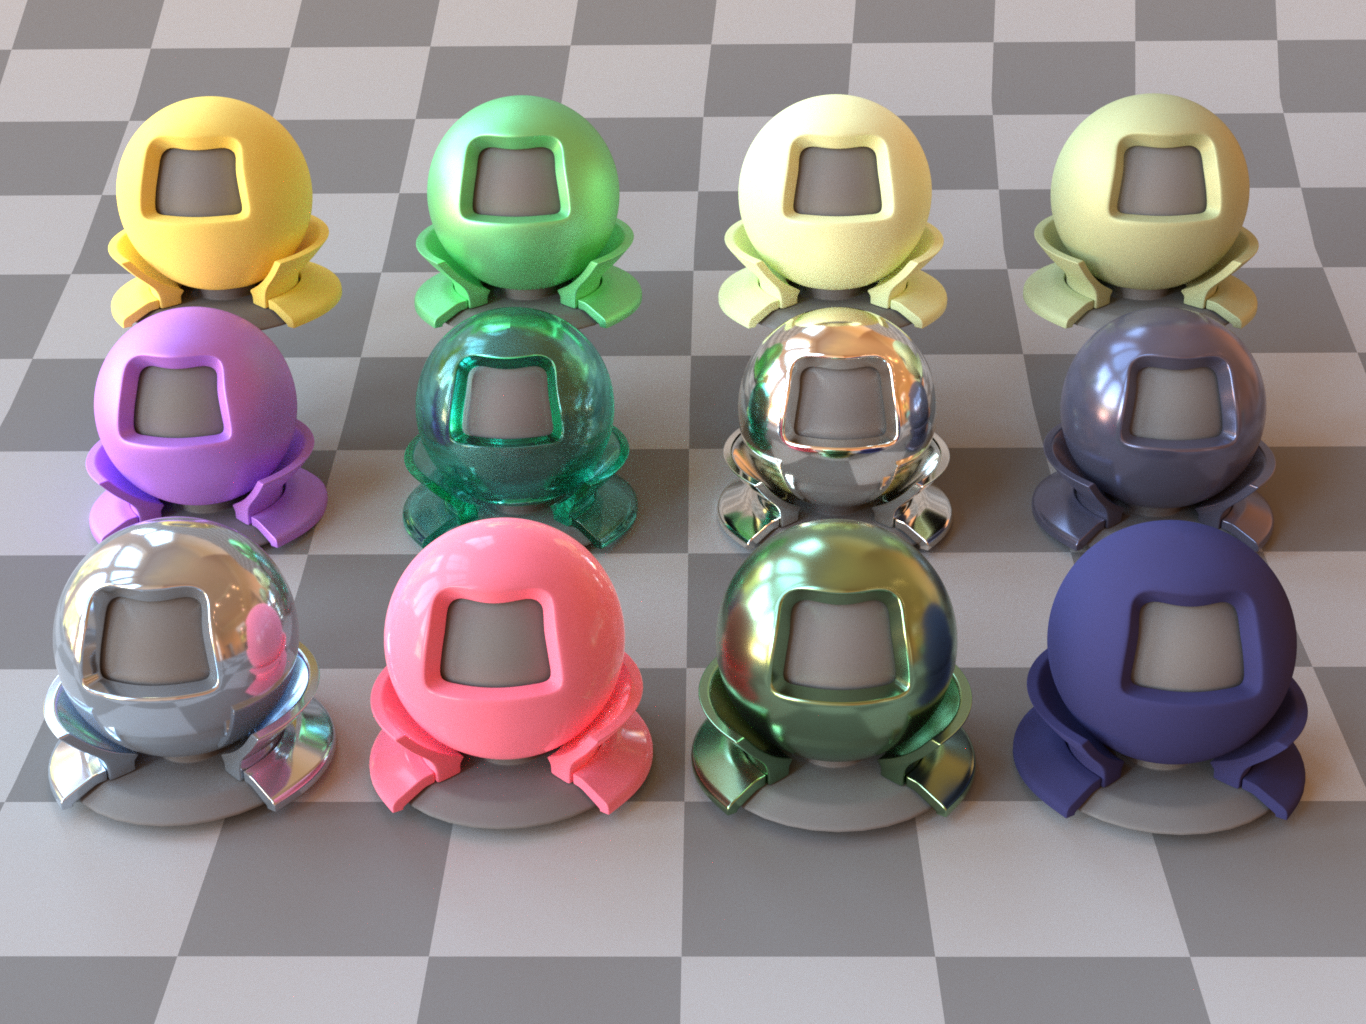
\includegraphics[width=\linewidth]{imgs/disney_bsdf.png}
    \caption{Disney principled BSDF~\cite{Burley:2012:PBS,Burley:2015:EDB} is a \emph{Uber shader} that can express a very wide range of materials.}
    \label{fig:gallery}
\end{figure}

In this homework we will implement a Bidirectional Scattering Distribution Function, called the \emph{Disney principled BSDF} (Figure~\ref{fig:gallery}), in lajolla. Disney principled BSDF is an attempt to have an one-size-fit-all solutions to cover most common materials using a single BSDF. It is \emph{principled} since it is (mostly) based on physical principles and observations from measured data~\cite{Matusik:2003:DRM}. However, physical correctness is not the utmost priority of the BSDF: it is a useful guideline for parametrizing the space of plausible materials for artistic expression. Ultimately, Disney BSDF is for making visual effects: as long as it makes graphics artists express what they want with least efforts, it achieves its goal. Disney BSDF is extremely influential since its inception in 2012. Nowadays, many commercial and non-commercial rendering engines feature a similar material: \href{https://docs.blender.org/manual/en/latest/render/shader_nodes/shader/principled.html}{Blender's principled BSDF}, \href{https://autodesk.github.io/standard-surface/}{Autodesk's Standard Surface}, \href{https://docs.unrealengine.com/4.26/en-US/RenderingAndGraphics/Materials/PhysicallyBased/}{Unreal Engine 4's physically-based materials}, \href{https://substance3d.adobe.com/tutorials/courses/the-pbr-guide-part-1}{Substance's physically-based shaders}, and \href{https://appleseed.readthedocs.io/projects/appleseed-maya/en/master/shaders/material/as_standard_surface.html}{Appleseed standard surface}, are all heavily inspired, if not directly borrowed from the Disney BSDF.

We will implement the Disney BSDF with a slight simplification: first, we won't implement the full volumetric absorption/scattering model (we will implement something similar in the next homework!). Second, we remove a sheen transmissive lobe to make sampling easier. When implementing the BSDF, feel free to reference code from internet. However, be aware that due to the ambiguity in the course note, all implementations I found are slightly different to each other, and some are flatout wrong\footnote{Even the implementation in pbrt appears to be wrong. See \href{https://github.com/mmp/pbrt-v3/issues/313}{here}.} I found the following links to be useful: \href{https://github.com/wdas/brdf/blob/main/src/brdfs/disney.brdf}{the official implementation of the BRDF} (lacks the transmission component and no sampling procedures), \href{https://github.com/mmp/pbrt-v3/blob/master/src/materials/disney.cpp}{pbrt's implementation}, \href{Joe Schutte's walkthrough}{https://schuttejoe.github.io/post/disneybsdf/}, \href{https://github.com/knightcrawler25/GLSL-PathTracer/blob/master/src/shaders/common/disney.glsl}{a GLSL implementation}, and \href{https://github.com/dfelinto/blender/blob/master/intern/cycles/kernel/shaders/node_principled_bsdf.osl}{Blender's open shading language implementation}. The model we will implement is the closest to Blender's version. You should read Burley's notes and presentations.\footnote{\url{https://blog.selfshadow.com/publications/s2012-shading-course/} and \url{https://blog.selfshadow.com/publications/s2015-shading-course/}}

A Disney BSDF is made of five components: a \textbf{diffuse} lobe that captures the base diffusive color of the surface, a \textbf{metallic} lobe that features major specular highlights, a \textbf{clearcoat} lobe that models the heavy tails of the specularity, a \textbf{sheen} lobe that addresses retroreflection, and a \textbf{glass} lobe that handles transmission. We will first implement each individual component, then we will combine all of them into a single material. 

\paragraph{Submission and grading.} Please send our teaching assistant Yan Xiao (yax010@ucsd.edu) a zip file including your code, and a text file (readme.txt) answering the questions below. We will grade your code by comparing individual ray queries with our reference code for the BSDF evaluation, we will check if your sampling code is consistent with the PDF, and we will eyeball your rendering to make sure everything looks fine. For the questions, as long as you say something plausible you will get full scores.

\paragraph{Notation and convention.} In the following, $\omega_{\text{in}}$ is the \emph{incoming} direction of the BSDF (usually represent the view direction), and $\omega_{\text{out}}$ is the \emph{outgoing} direction of the BSDF (usually represent the light direction), both pointing \emph{outwards} from the surface. $n$ is the shading normal, $h$ is the half-vector $h = \frac{\omega_{\text{in}} + \omega_{\text{out}}}{\|\omega_{\text{in}} + \omega_{\text{out}}\|}$. All of our BSDF include the cosine term $|n \cdot \omega_{\text{out}}|$. All parameters of Disney BSDF are normalized within $[0, 1]$.

\section{Diffuse}
\begin{figure}
	\caption{Diffuse rendering}
\end{figure}

By looking at the MERL measured BRDF~\cite{Matusik:2003:DRM}, Burley found that at grazing retroreflection (when the half vector is roughly orthogonal to the normal), smooth materials (materials that are more specular) tend to have their reflectance dropped, and rough materials tend to have a peak at the grazing angle. The dropped reflectance can be predicted by Fresnel reflection: at grazing angles, (dielectric) Fresnel equation predicts low transmittance and less lights are scattered inside the surfaces and thus less diffusion. Thus they design the following diffuse BRDF based on a modified version of the Schlick Fresnel approximation~\cite{Schlick:1994:IBM}:
\begin{equation}
	f_{\text{baseDiffuse}} = \frac{\text{baseColor}}{\pi}
	F_D(\omega_{\text{in}}) F_D(\omega_{\text{out}}) |n \cdot \omega_{\text{out}}|,
\end{equation}
where
\begin{equation}
\begin{aligned}
F_D(\omega) &= \left(1 + (F_{D90} - 1) (1 - |n \cdot \omega|)^5 \right) \\
F_{D90} &= \frac{1}{2} + 2 \text{roughness} |h \cdot \omega_{\text{out}}|^2.
\end{aligned}
\end{equation}

When $\text{roughness} = 0$ (smooth materials), at grazing view angle $|n \cdot \omega_{\text{in}}| \approx 0$, and at grazing lighting angle $|n \cdot \omega_{\text{out}}| \approx 0$, thus the BSDF attenuates the diffuse response by a factor of $\frac{1}{2}$ for each $F_D$ term (modelling the Fresnel reflection). At high roughness ($\text{roughness} \approx 1$), at retroreflection, $\omega{\text{out}} \approx \omega{\text{in}}$, thus $h \cdot \omega_{\text{out}} \approx 1$, and the BSDF reproduces the peak retroreflection observed in the MERL data by multiplying $2.5$ for each $F_D$ term.

In addition to the base diffuse model, the diffuse component of Disney BSDF also blends it with a subsurface scattering lobe for surfaces with strong multiple scattering inside like skin, milk, or marble. In the 2015 version of the Disney BSDF, they simulate \emph{real} subsurface scattering that requires volumetric path tracing to simulate the scattering, but this is too much work for the first homework. Instead, we follow the 2012 version and use a BRDF approximation of the subsurface scattering by modifying the Lommel-Seeliger law:
\begin{equation}
	f_{\text{subsurface}} = \frac{1.25 \text{baseColor}}{\pi} \left(
	F_{SS}(\omega_{\text{in}}) F_{SS}(\omega_{\text{out}}) \left(\frac{1}{|n \cdot \omega_{\text{in}}| + |n \cdot \omega_{\text{out}}|} - 0.5 \right) + 0.5 \right).
\end{equation} 

See \href{https://phys.libretexts.org/Bookshelves/Astronomy__Cosmology/Book%3A_Planetary_Photometry_(Tatum_and_Fairbairn)/03%3A_A_Brief_History_of_the_Lommel-Seeliger_Law/3.01%3A_A_Brief_History_of_the_Lommel-Seeliger_Law#:~:text=Description.,physical%20model%20of%20diffuse%20reflection.&text=Thus%2C%20of%20this%20diffuse%20scattered,emerging%20as%20diffuse%20reflected%20radiation.}{here} for a nice sketch of derivation of the Lommel-Seeliger law (brought to graphics by Hanrahan and Kruger~\cite{Hanrahan:1993:RLS}). The $\frac{1}{|n \cdot \omega_{\text{in}}| + |n \cdot \omega_{\text{out}}|}$ term models the volumetric absorption of the scattering media below the surface.

The final diffuse BRDF is:
\begin{equation}
	f_{\text{diffuse}} = (1 - \text{subsurface}) f_{\text{baseDiffuse}} + \text{subsurface} f_{\text{subsurface}},
	\label{eq:f_diffuse}
\end{equation}
where $\text{subsurface}$ is a parameter.

Note that the physical model here is a dielectric coating on top of a diffusive scattering media (similar to the \lstinline{roughplastic} material in lajolla/Mitsuba), but $f_{\text{diffuse}}$ does not model the specular reflection of the dielectric coating. We will include the specular reflection in the final assembly.

\paragraph{Task (10\%).} You will implement the \lstinline{DisneyDiffuse} BRDF (Equation~\ref{eq:f_diffuse})
\begin{lstlisting}
// in material.h
struct DisneyDiffuse {
    Texture<Spectrum> base_color;
    Texture<Real> roughness;
    Texture<Real> subsurface;
};
\end{lstlisting}

You need to implement the following three functions in \lstinline{materials/disney_diffuse.inl}:
\begin{lstlisting}
Spectrum eval_op::operator()(const DisneyDiffuse &bsdf) const;
Real pdf_sample_bsdf_op::operator()(const DisneyDiffuse &bsdf) const;
std::optional<BSDFSampleRecord> sample_bsdf_op::operator()(const DisneyDiffuse &bsdf) const;
\end{lstlisting}

For sampling, we will simply use a cosine hemisphere sampling. Look at \lstinline{materials/lambertian.inl} to see how it is done. Feel free to copy paste the code and modify anything. Also notice how the Lambertian BRDF implementation handles the discrepancy between geometry normals and shading normals.

Try out \lstinline{./lajolla ../scenes/disney_diffuse.xml} to see how the material look like. Play with the parameters.

\paragraph{Questions (5\%).} Answer these questions in a text file:
\begin{enumerate}
	\item Compare the two BRDFs with a Lambertian BRDF: what differences do you see? Why?
	\item Compare the base diffuse BRDF ($f_{\text{baseDiffuse}}$) with the subsurface BRDF ($f_{\text{subsurface}}$) by playing with the subsurface parameter. What differences do you see? Why? In what lighting condition does the base diffuse BRDF differ the most from the subsurface BRDF?
\end{enumerate}

\section{Metal}
\begin{figure}
	\caption{Metal rendering}
\end{figure}

For specular reflection, Burley uses a standard Cook-Torrance microfacet BRDF~\cite{Cook:1982:RMC}:
\begin{equation}
f_{\text{metal}} = \frac{F_m D_m G_m}{4 |n \cdot \omega_{\text{in}}|},\footnote{The $|n \cdot \omega_{\text{out}}|$ term in the denominator cancels out with the cosine.}
\label{eq:f_metal}
\end{equation}
where $F_m$ is the Fresnel reflection, $D_m$ is the probability density of the distribution of a microfacet normal, and $G_m$ is the masking-shadowing term~\cite{Heitz:2014:UMF} that models the occlusion between microfacets.

For the Fresnel term $F_m$, Burley uses the Schlick approximation:
\begin{equation}
F_m = \text{baseColor} + (1 - \text{baseColor}) (1 - |n \cdot \omega_{\text{out}}|^5).
\end{equation}
The reason why they use an approximation instead of the true Fresnel equation is not just for the performance. For metallic surfaces, or \emph{conductors}, Fresnel equation requires us to have the complex index of refraction of the conductor for each wavelength. This parameter is not only unintuitive, but nor is it physically accurate when we only consider the RGB spectrum.\footnote{See \href{http://renderwonk.com/publications/mam2019/}{``Fresnel Equations Considered Harmful''} by Naty Hoffman. \href{https://www.youtube.com/watch?v=kEcDbl7eS0w}{Here} is his presentation video.} 

For the normal distribution function $D_m$, Burley uses the anisotropic Trowbridge-Reitz distribution~\cite{Trowbridge:1975:AIR}, popularized by Walter et al.~\cite{Walter:2007:MMR} in graphics and it is known as \emph{GGX} (Ground Glass X):
\begin{equation}
D_m = \frac{1}{\pi \alpha_x \alpha_y \left(\frac{h_l.x^2}{\alpha_x^2} + \frac{h_l.y^2}{\alpha_y^2} + h_l.z^2\right)^2},
\end{equation}
where $h_l$ is the half vector projected to the local frame. Trowbridge-Reitz distribution was found to be fitting the MERL measured data excellently thanks to its heavy tails compared to a Gaussian or a cosine (some materials have even longer tails, and those will be modelled by the clearcoat component later). 

$\alpha_x, \alpha_y$ are parameters for modelling the smoothness of the material. If we directly use these parameters, we need very small $\alpha$ to represent highly specular materials. Burley found that the following mapping is more intuitive:
\begin{equation}
\begin{aligned}
\text{aspect} &= \sqrt{1 - 0.9 \text{anisotropic}} \\
\alpha_x &= max(\alpha_{\text{min}}, \text{roughness} \cdot \text{roughness} / \text{aspect}) \\
\alpha_y &= max(\alpha_{\text{min}}, \text{roughness} \cdot \text{roughness} \cdot \text{aspect})
\end{aligned},
\end{equation}
where $\text{anisotropic}$ and $\text{roughness}$ are the parameters.

Given a normal distribution function and a microfacet configuration, it is possible to derive the average occlusion factor $G_m$ given a viewing angle~\cite{Heitz:2014:UMF}. Burley uses the Smith model, which enables a closed-form solution under the assumption that all the microfacets are independently oriented:
\begin{equation}
\begin{aligned}
G_m &= G(\omega_{\text{in}}) G(\omega_{\text{out}}) \\
G(\omega) &= \frac{1}{1 + \Lambda(\omega)} \\
\Lambda(\omega) &= \frac{\sqrt{1 + \frac{\left(\omega_l.x \cdot \alpha_x\right)^2 + \left(\omega_l.y \cdot \alpha_y\right)^2}{\omega_l.z^2}} - 1}{2}
\end{aligned}.
\end{equation}

Combining all of these, and you will get a nice metallic BRDF.

\paragraph{Task (10\%).} You will implement the \lstinline{Disney} BRDF (Equation~\ref{eq:f_metal})
\begin{lstlisting}
// in material.h
struct DisneyMetal {
    Texture<Spectrum> base_color;
    Texture<Real> roughness;
    Texture<Real> anisotropic;
};
\end{lstlisting}

You need to implement the following three functions in \lstinline{materials/disney_metal.inl}:
\begin{lstlisting}
Spectrum eval_op::operator()(const DisneyMetal &bsdf) const;
Real pdf_sample_bsdf_op::operator()(const DisneyMetal &bsdf) const;
std::optional<BSDFSampleRecord> sample_bsdf_op::operator()(const DisneyMetal &bsdf) const;
\end{lstlisting}

For sampling, we will use the visible normal sampling developed by Heitz~\cite{Heitz:2018:SGD}, which importance samples $D_m G(\omega_{\text{in}})$. See Heitz's presentation \href{https://jcgt.org/published/0007/04/01/slides.pdf}{slides} for a really nice illustration of the method. This sampling is also used in the \lstinline{roughplastic} material in lajolla, so you might want to look at it as well.

Try out \lstinline{./lajolla ../scenes/disney_metal.xml} to see how the material look like. Play with the parameters.

\paragraph{Questions (5\%).} Answer these question(s) in a text file:
\begin{enumerate}
	\item Compare \lstinline{DisneyMetal} with the \lstinline{roughplastic} material. What differences do you see?
\end{enumerate}

\bibliographystyle{plain}
\bibliography{refs}

\end{document}